\title{ALPSチュートリアル -- ALPSの概要}

\begin{document}

\begin{frame}
  \titlepage
\end{frame}

\section*{Outline}
\begin{frame}
  \tableofcontents
\end{frame}


\section{チュートリアルの概要}

\begin{frame}{ALPSチュートリアル スタッフ}
  \begin{itemize}
  \item 講師
    \begin{itemize}
    \item 藤堂眞治 (東大物性研) \ \href{mailto:wistaria@issp.u-tokyo.ac.jp}{wistaria@issp.u-tokyo.ac.jp}
    \item 松尾春彦 (RIST) \ \href{mailto:halm@rist.or.jp}{halm@rist.or.jp}
    \item 五十嵐 亮 (東大物性研) \ \href{mailto:rigarash@issp.u-tokyo.ac.jp}{rigarash@issp.u-tokyo.ac.jp}
    \end{itemize}
  \item 主催
    \begin{itemize}
    \item CMSI: 計算物質科学イニシアティブ \url{http://cms-initiative.jp/}
    \end{itemize}
  \item 共催
    \begin{itemize}
    \item RIST: 一般財団法人 高度情報科学技術研究機構 \url{http://www.rist.or.jp/}
    \end{itemize}
  \end{itemize}
\end{frame}

\begin{frame}
  \frametitle{チュートリアルの流れ}
  \begin{tabular}{|l|l|c|c|c|}
        \hline
        Getting Started & {\tt 00\_gettingstarted} & {\footnotesize\color{red} ○} & {\footnotesize\color{blue} ○} & {\footnotesize\color{green} ○} \\
        \hline
        ALPSの概要 & {\tt 01\_overview} & {\footnotesize\color{red} ◎} & {\footnotesize\color{blue} ◎} & {\footnotesize\color{green} ◎} \\
        \hline
        ALPSライブラリ & {\tt 02\_library} & {\footnotesize\color{red} ○} & {\footnotesize\color{blue} ◎} & {\footnotesize\color{green} ◎} \\
        \hline
        アプリケーション実習(1) & {\tt 03\_tutorial} & {\footnotesize\color{red} ◎} & {\footnotesize\color{blue} ○} & {\footnotesize\color{green} ◎} \\
        \hline
        Python入門 & {\tt 04\_python} & {\footnotesize\color{red} ○} & {\footnotesize\color{blue} ◎} & {\footnotesize\color{green} ◎} \\
        \hline
        ALPS Phthon入門 & {\tt 05\_pyalps} & {\footnotesize\color{red} ○} & {\footnotesize\color{blue} ◎} & {\footnotesize\color{green} ◎} \\
        \hline
        Matplotlib入門 & {\tt 06\_matplotlib} & {\footnotesize\color{red} ○} & {\footnotesize\color{blue} ○} & {\footnotesize\color{green} ◎} \\
        \hline
        アプリケーション実習(2) & & {\footnotesize\color{red} ◎} & {\footnotesize\color{blue} } & {\footnotesize\color{green} ◎} \\
        \hline
        アプリケーションのALPS化 & {\tt 07\_alpsize} & {\footnotesize\color{red} } & {\footnotesize\color{blue} ◎} & {\footnotesize\color{green} ◎} \\
        \hline
        ALPSのインストール & {\tt 08\_installation} & {\footnotesize\color{red} ○} & {\footnotesize\color{blue} ◎} & {\footnotesize\color{green} ◎} \\
        \hline
  \end{tabular}
  
  {\footnotesize\color{red} ○}: ユーザコース、{\footnotesize\color{blue} ○}: 開発者コース {\footnotesize\color{green} ○}: 集中コース
\end{frame}

\begin{frame}
  \frametitle{ALPSチュートリアルの目標}
  \begin{itemize}
    \setlength{\itemsep}{1em}
    \item ALPSの概要を知る \ [{\footnotesize\color{red} ○}{\footnotesize\color{blue} ○}{\footnotesize\color{green} ○}]
    \item ALPSアプリケーションの実行方法を学ぶ  \ [{\footnotesize\color{red} ○}{\footnotesize\color{blue} ー}{\footnotesize\color{green} ○}]
    \item ALPS Pythonツールを使った結果の解析方法を学ぶ  \ [{\footnotesize\color{red} ○}{\footnotesize\color{blue} ー}{\footnotesize\color{green} ○}]
    \item ALPSライブラリの仕組みを学ぶ \ [{\footnotesize\color{red} ー}{\footnotesize\color{blue} ○}{\footnotesize\color{green} ○}]
    \item ユーザアプリケーションの作成方法を学ぶ  \ [{\footnotesize\color{red} ー}{\footnotesize\color{blue} ○}{\footnotesize\color{green} ○}]
    \item (ALPSチュートリアルの問題点を洗い出し改良する) \ [{\footnotesize\color{red} ◎}{\footnotesize\color{blue} ◎}{\footnotesize\color{green} ◎}] 
  \end{itemize}
\end{frame}

\section{量子格子模型とは?}
\begin{frame}{量子格子模型: Quantum Lattice Models}
  \begin{columns}[T]
    \begin{column}{.8\textwidth}
      \begin{itemize}
      \item 量子スピン模型(XXZ模型) \begin{equation*} {\cal H} = \frac{J^{xy}}{2}
        \sum_{\langle i,j \rangle} (S^+_i S^-_j + S^-_i S^+_j) + J^z
        \sum_{\langle i,j \rangle} S^z_i S^z_j \end{equation*}
      \item Hubbard模型 \begin{equation*} {\cal H} = -t \sum_{\langle i,j \rangle \sigma}
        (c^\dagger_{i\sigma} c_{j\sigma} + \mbox{h.c.}) + U \sum_{i}
        n_{i\uparrow} n_{i\downarrow} \end{equation*}
      \item t-J模型 \begin{equation*} {\cal H} = -t \sum_{\langle i,j \rangle \sigma}
        (c^\dagger_{i\sigma} c_{j\sigma} + \mbox{h.c.}) + J \sum_{i,j}
        ({\bf S}_i \cdot {\bf S}_j - n_{i} n_{j} / 4) \end{equation*}
      \end{itemize}
    \end{column}
    \begin{column}{.2\textwidth}
      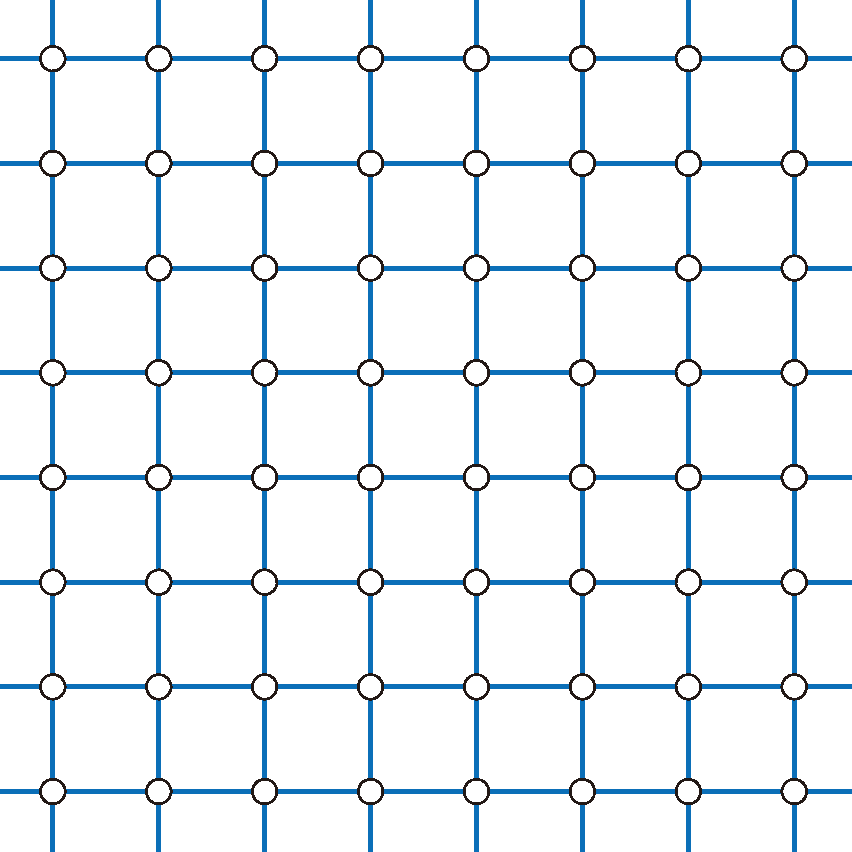
\includegraphics[width=\textwidth]{square.pdf}
    \end{column}
  \end{columns}
\end{frame}

\begin{frame}{なぜQLMを考えるのか?}
  \begin{columns}[T]
    \begin{column}{.2\textwidth}
      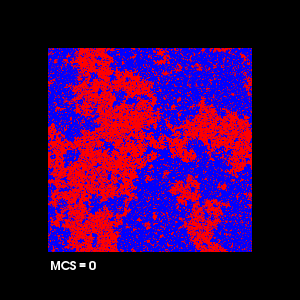
\includegraphics[width=\textwidth]{ising-tc.png} \\
      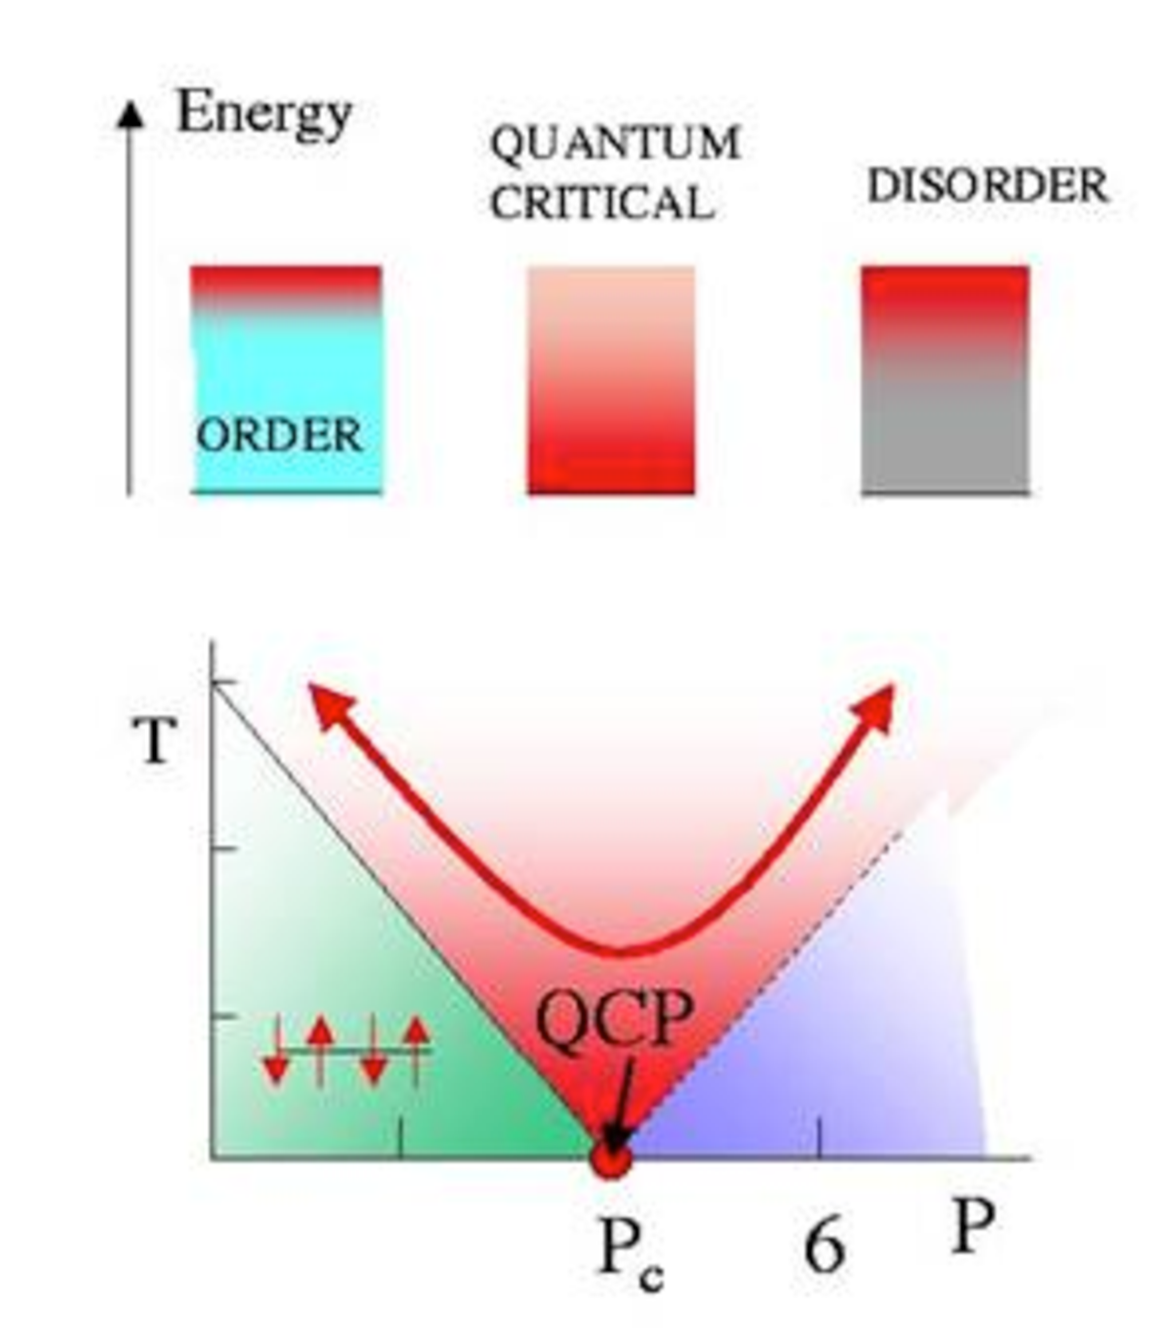
\includegraphics[width=\textwidth]{qcp.pdf}
    \end{column}
    \begin{column}{.8\textwidth}
      \begin{itemize}
        %\setlength{\itemsep}{1em}
      \item 量子多体系における強相関効果
        \begin{itemize}
        \item さまざまな秩序状態
        \item 量子的に強くゆらいだ相: 量子液体, スピンギャップ相
        \item 量子相転移, 量子臨界現象
        \end{itemize}
      \item 量子統計物理におけるユニバーサリティー
        \begin{itemize}
        \item 量子臨界現象は系の次元, 秩序変数の対称性などにしか依存しない
        \item 量子臨界現象特有のユニバーサリティークラスの探索
        \end{itemize}
      \item 新しい計算物理学的手法の発展
        \begin{itemize}
        \item 量子モンテカルロ法, DMRG, DMFT, テンソルネットワーク, など
        \end{itemize}
      \end{itemize}
    \end{column}
  \end{columns}
\end{frame}

%\begin{frame}{実験室で実現されているQLM}
%\end{frame}

%\begin{frame}{Finite-size scaling analysis}
%\end{frame}
  
\section{ALPSプロジェクト}

\begin{frame}
  \frametitle{ALPSプロジェクトの目標}
  \begin{itemize}
    \setlength{\itemsep}{1em}
  \item 量子統計物理分野の現状
    \begin{itemize}
    \item 研究グループ毎に異なるコードを開発
    \item シミュレーションを行う模型毎に異なる実装
    \item アルゴリズムはますます複雑なりソフトウェア開発が長期化
    \item 可搬性・互換性のない入出力形式
    \end{itemize}
  \item ALPSプロジェクトの目標
    \begin{itemize}
    \item 最新のアルゴリズムを用いた``community code''の開発
    \item 大規模並列計算などのためのC++ライブラリ・フレームワーク開発
    \item 統一入出力形式の提案とそれにもとづくデータ解析ツールの作成
    \item 計算物理の専門家だけでなく, 理論家・実験家にも使えるシミュレーションソフトウェア
    \end{itemize}
  \end{itemize}
\end{frame}

\begin{frame}{ALPSとは?}
  ALPS = Algorithms and Libraries for Physics Simulations
  %\begin{columns}[T]
    %\begin{column}{.7\textwidth}
      \begin{itemize}
      \item 量子スピン系, 電子系など強相関量子格子模型のシミュレーショ
        ンためのオープンソースソフトウェアの開発を目指す国際共同プロジェ
        クト
        %\begin{itemize}
        \item ALPSライブラリ = C++による格子模型のための汎用ライブラリ群
        \item ALPSアプリケーション = 最新のアルゴリズムに基づくアプリケーション群: QMC, DMRG, ED, DMFT等
        \item ALPSフレームワーク = 汎用入出力形式, 解析ツール, スケジュー
          ラなど, 大規模並列シミュレーションのための環境
        %\end{itemize}
      \end{itemize}
    %\end{column}
    %\begin{column}{.3\textwidth}
      %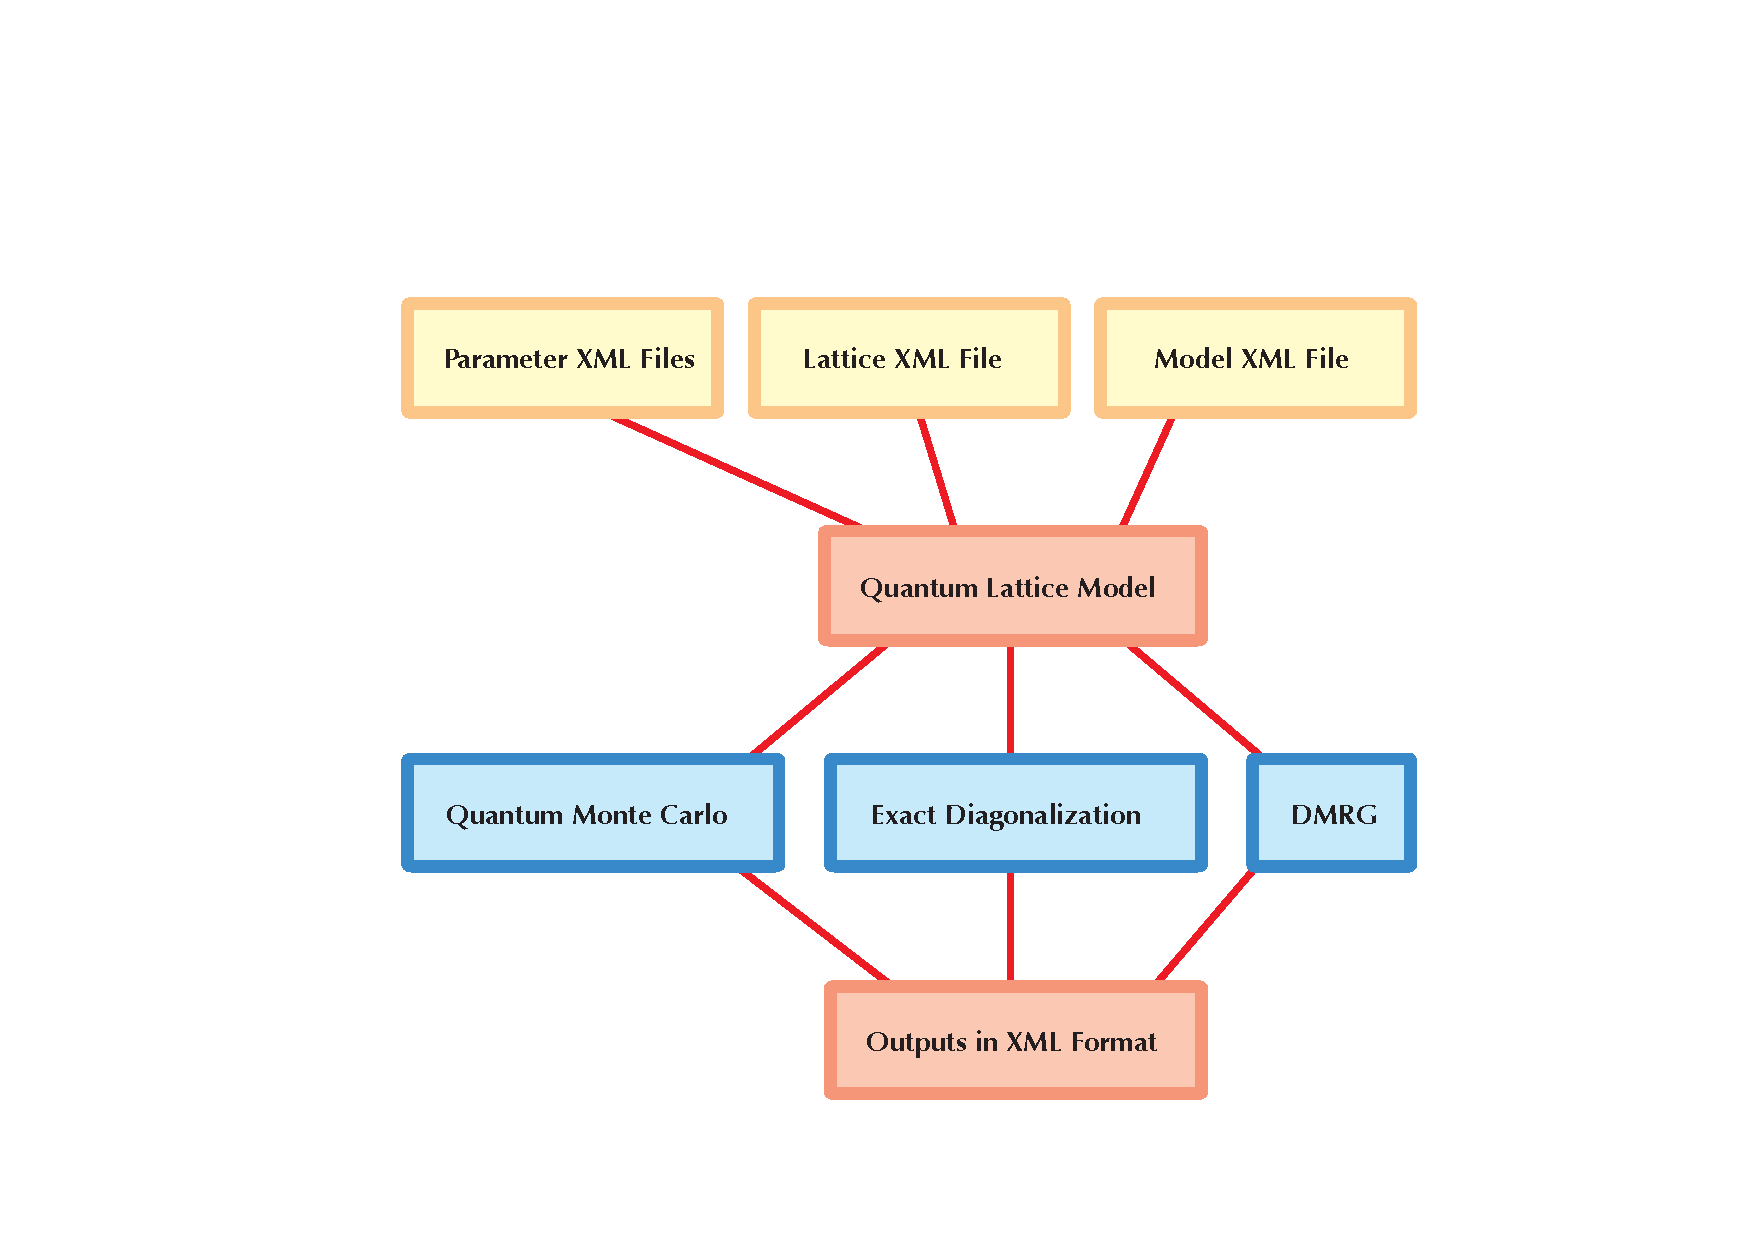
\includegraphics[width=1.2\textwidth]{simulation.pdf}
    %\end{column}
  %\end{columns}
\end{frame}

\begin{frame}{ターゲット・オーディエンス}
  \begin{itemize}
    \setlength{\itemsep}{1em}
  \item 実験家
    \begin{itemize}
    \item 物質のモデリングにソフトウェアパッケージを利用
    \item 実験結果とシミュレーション結果のフィッティングにより, 相互作用定数などを決定
    \end{itemize}
  \item 理論家
    \begin{itemize}
    \item 理論的なアイデアのチェックに使いやすい整備されたコードを利用
    \item 自前のコードのデバッグに
    \item 新しいコード開発の基盤としての利用
    \end{itemize}
  \item 計算機科学者, 学生, $\cdots$
  \end{itemize}
\end{frame}

\section{ALPSによるシミュレーション}

\begin{frame}{ALPSによるシミュレーション --- ワークフロー}
  \begin{center}
    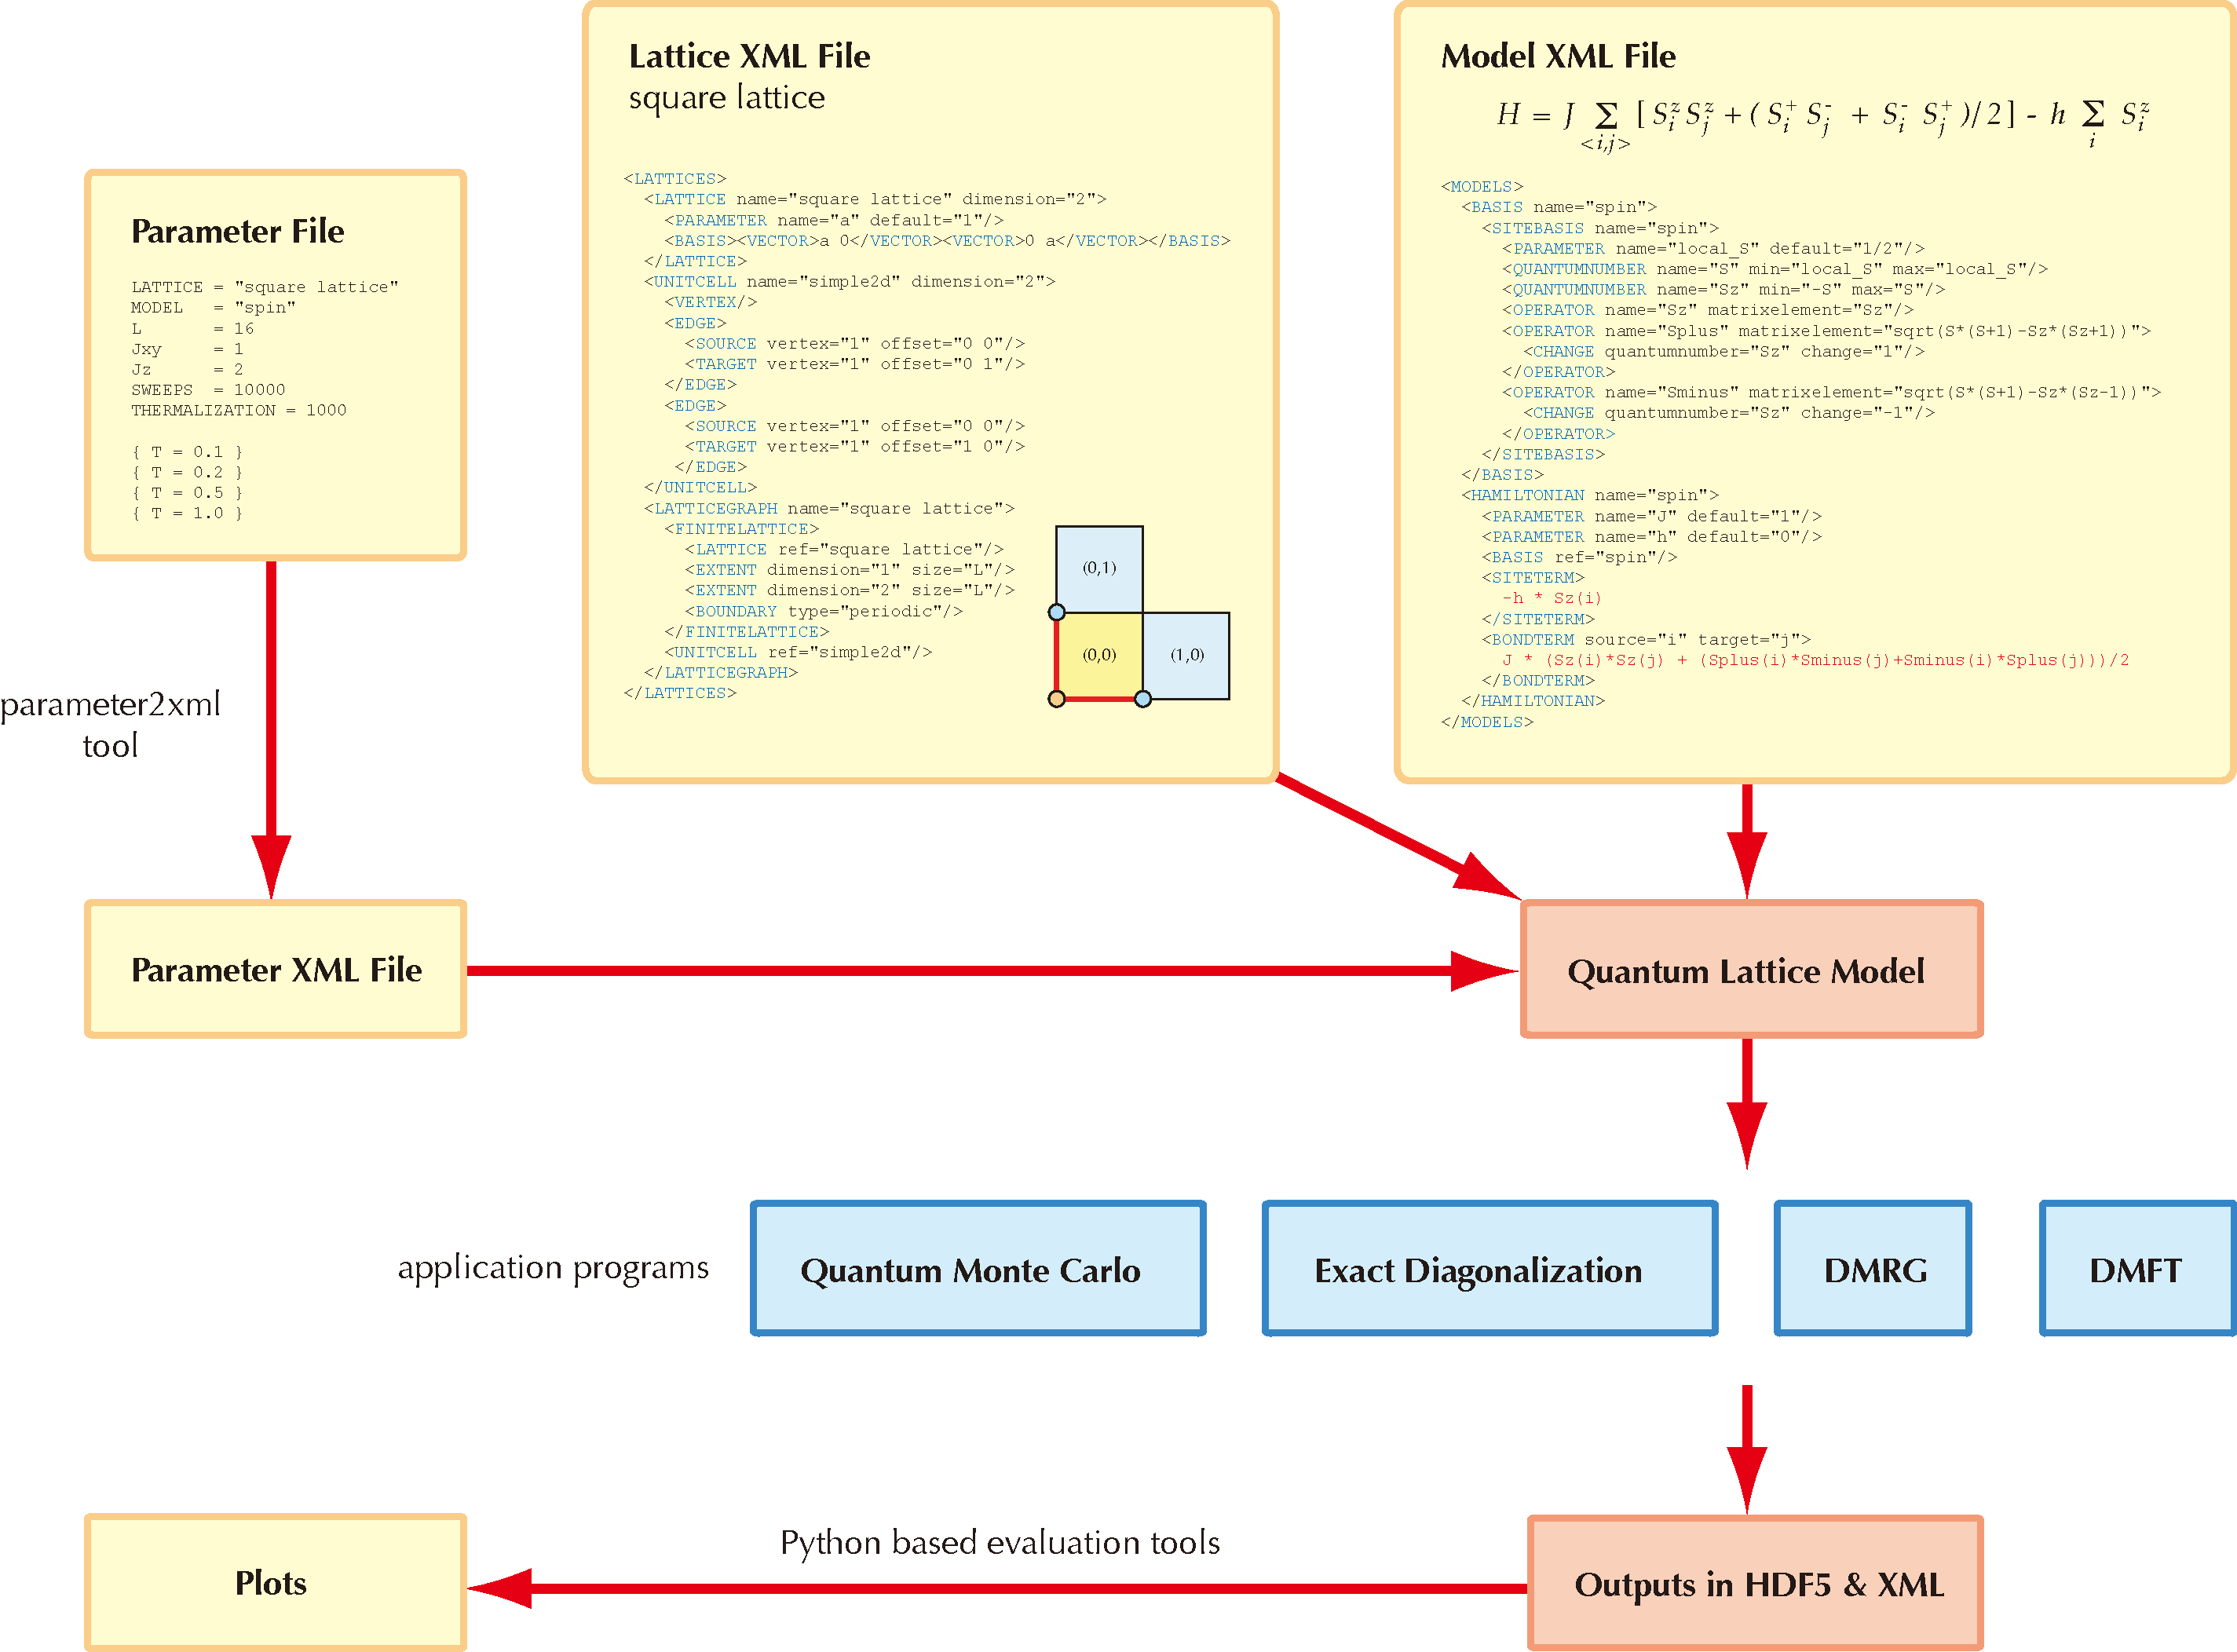
\includegraphics[height=0.8\textheight]{workflow.pdf}
  \end{center}
\end{frame}

\begin{frame}{ALPSの階層構造}
  \begin{center}
    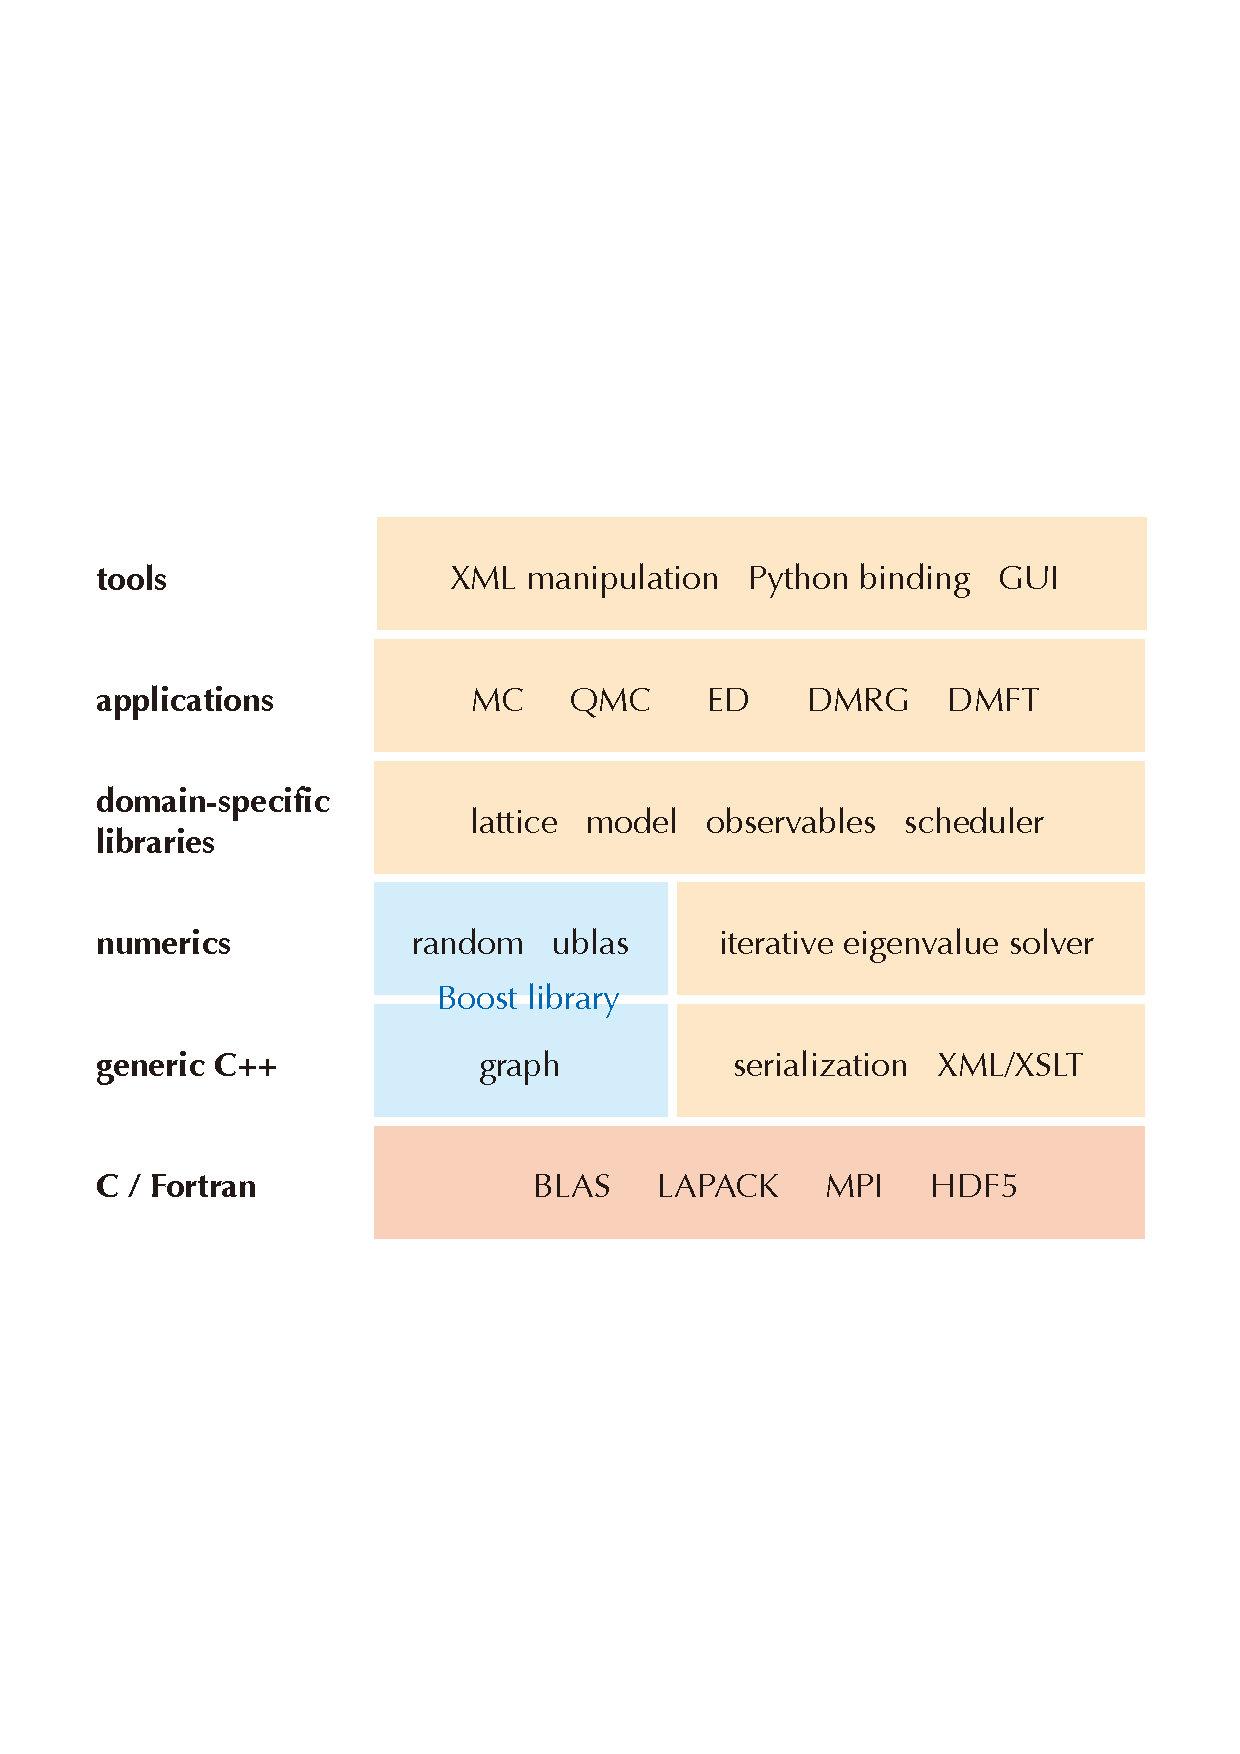
\includegraphics[height=0.65\textheight]{hierarchy.pdf}
  \end{center}
\end{frame}

\section{ALPSの開発}

\begin{frame}
  \frametitle{基盤となる技術}
  \begin{itemize}
    \setlength{\itemsep}{1em}
  \item C++によるジェネリック・プログラミング
    \begin{itemize}
    \item C++標準テンプレートライブラリ
    \item Boost C++ ライブラリ \url{http://www.boost.org/}
    \item ALPS独自のクラス, ジェネリック・アルゴリズムを実装
    \item 柔軟性, 再利用性, 高信頼性, 高性能を同時に達成
    \end{itemize}
  \item XML, HDF5による入出力
    \begin{itemize}
    \item 可搬性, 自己記述性, 変換が容易
    \end{itemize}
  \item 量子格子模型に対する最新のシミュレーション手法
  \end{itemize}
\end{frame}

\begin{frame}
  \frametitle{なぜC++を使うのか?}
  \begin{columns}{T}
    \begin{column}{.5\textwidth}
      \centering 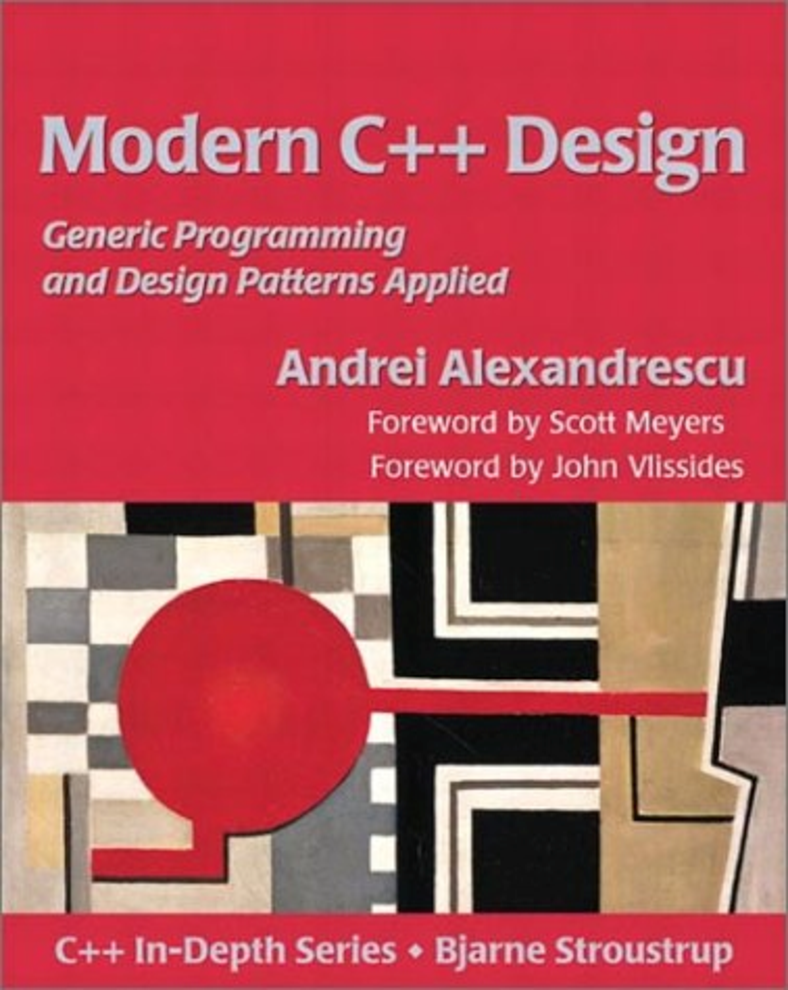
\includegraphics[width=4.5cm]{modern-cxx.pdf}
    \end{column}
    \begin{column}{.5\textwidth}
      \centering 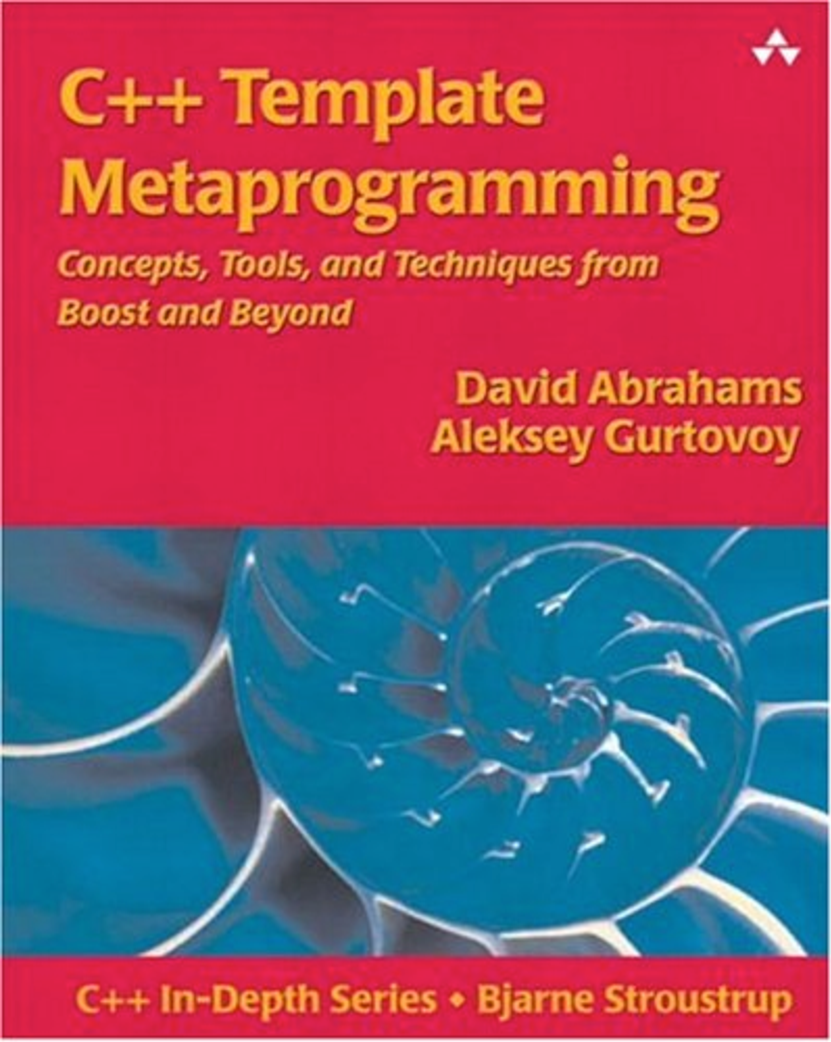
\includegraphics[width=4.5cm]{cxx-template.pdf}
    \end{column}
  \end{columns}
\end{frame}

\begin{frame}
  \frametitle{ALPSの歴史}
  \begin{itemize}
  \item 1990年代中頃 ALPSの前身となる PALM C++, DMRG, looper などが開発される
  \item 2002年 ALPSプロジェクト始動
  \item 2004年 バージョン1.0, 第1回 Users Workshop
  \item 2010年 バージョン2.0
  \item 2011年7月現在
    \begin{itemize}
      \item ソースコード: C++ 310,000行, Python 19,000行, Fortran 10,000行
      \item 開発者: 約30名(7ヶ国)
    \end{itemize}
  \end{itemize}
\end{frame}

\begin{frame}
  \frametitle{ALPSの開発者 (2011.5現在)}
  \begin{columns}[T]
    \begin{column}{.33\textwidth}
      \begin{itemize}
      \item Austria
        \begin{itemize}
        \item H. G. Evertz
        \end{itemize}
      \item France
        \begin{itemize}
        \item O. Parcollet
        \end{itemize}
      \item Germany
        \begin{itemize}
        \item S. Fuchs
        \item G. Guertler
        \item D. Koop
        \item U. Shollw\"ock
        \item S. Trebst
        \item S. Wessel
        \end{itemize}
      \item Poland
        \begin{itemize}
        \item G. Pawlowski
        \end{itemize}
      \end{itemize}
    \end{column}
    \begin{column}{.35\textwidth}
      \begin{itemize}
      \item Switerland
        \begin{itemize}
        \item B. Bauer
        \item L. Gamper
        \item J. Gukelberger
        \item A. Hehn
        \item S. V. Isakov
        \item P. N. Ma
        \item P. Mates
        \item J. D. Picon
        \item L. Pollet
        \item B. Surer
        \item M. Troyer
        \item P. Werner
        \end{itemize}
      \end{itemize}
    \end{column}
    \begin{column}{.35\textwidth}
      \begin{itemize}
      \item Japan
        \begin{itemize}
        \item 五十嵐 亮
        \item 松尾春彦
        \item 藤堂眞治
        \end{itemize}
      \item USA
        \begin{itemize}
        \item L. D. Carr
        \item A. Feiguin
        \item J. Freire
        \item E. Gull
        \item E. Santos
        \item V. W. Scarlola
        \item C. Silva
        \item M. L. Wall
        \end{itemize}
      \end{itemize}
    \end{column}
  \end{columns}
\end{frame}

\begin{frame}
  \frametitle{開発のためのインフラストラクチャ}
  \begin{itemize}
  \item ソースコードの規模, 開発体制が大きくなると今までの方法では破綻する
  \item 開発・サポートのためのツールを一から作りあげるのは非現実的
  \item フリーソフトウェアの利用
    \begin{itemize}
    \item ビルドシステム: CMake
    \item ソースコードの管理: Subversion
    \item プロジェクト管理・バグ追跡: Trac
    \item ドキュメント作成: MediaWiki
    \item メーリングリスト: Mailman
    \end{itemize}
  \item Linux ワークステーションが1台あれば, これらの環境を整えるのは現在では比較的容易
  \end{itemize}
\end{frame}

\begin{frame}
  \frametitle{ビルドシステム: CMake}
  \begin{itemize}
    \setlength{\itemsep}{1em}
  \item Makefileを生成するためのユーティリティー (configureスクリプトに対応)
    \begin{itemize}
    \item Windows の Visual C++ 用ソリューションファイル, Mac OS X の Xcode 用プロジェクトファイルの生成も可能
    \end{itemize}
  \item 設定は CMakeLists.txt に記述する
  \item テスト(CTest)やバイナリ配布(CPack)の機能もある
  \item ファイルの依存関係の自動検出
  \end{itemize}
\end{frame}

\begin{frame}
  \frametitle{VCS (Version Control System)によるソース管理: Subversion}
  \begin{itemize}
  \item 開発者が複数になると, ディレクトリ名やログファイルによるバージョン管理はすぐに破綻する
  \item ソースコードをサーバー上で一括管理
    \begin{itemize}
    \item ネットワーク経由でソースを check out/check in
    \end{itemize}
  \item 更新毎に一意なバージョン番号を付与
  \item 全ての修正履歴を保存
  \item 複数人が同時に更新した場合に衝突を回避するしくみ
  \item ブランチ・マージ・タグ付けなどが可能
  \item 開発者が一人, 公開の予定がない場合でも積極的に使うべき
  \end{itemize}
\end{frame}

\begin{frame}
  \frametitle{BTS (Bug Tracking System) の利用: Trac}
  \begin{itemize}
    \setlength{\itemsep}{1em}
  \item プロジェクト管理とバグ追跡のためのツール
  \item Web ブラウザからアクセス・操作
    \begin{itemize}
    \item 開発者の情報共有のための wiki
    \item Subversion との連携 (ソース, 修正履歴の web 上での閲覧)
    \item プロジェクト管理 (ロードマップ, マイルストーンの管理)
    \item チケットシステム: バグやタスクの登録, 担当者の決定, 修正状況の追跡
    \end{itemize}
  \end{itemize}
\end{frame}

\begin{frame}
  \frametitle{Wikiによるマニュアル作成: MediaWiki}
  \begin{itemize}
  \item もともとはウィキペディアのために開発された
  \item Wiki とは?
    \begin{itemize}
    \item Webブラウザを利用してWeb文書を書き換えるシステム
    \item ネットワーク上のどこからでも書き換えができる
    \item 共同作業が容易
    \item Webブラウザがあれば編集作業が行える
    \item HTMLよりも簡潔な書式
    \item 文書間のリンクの作成が容易
    \end{itemize}
  \item ALPS Wiki のコンテンツ
    \begin{itemize}
    \item ニュース, インストール方法, ALPSに関連する論文, 発表資料, ライブラリリファレンスマニュアル, チュートリアル
    \end{itemize}
  \end{itemize}
\end{frame}

\begin{frame}
  \frametitle{メーリングリストの活用: Mailman}
  \begin{itemize}
    \setlength{\itemsep}{1em}
  \item 開発者メーリングリスト
    \begin{itemize}
    \item 開発方針に関する意見交換, リリーススケジュール調整, 担当者調整等
    \item Trac チケットの変更ログも自動的にここに流れる
    \end{itemize}
  \item ユーザメーリングリスト
    \begin{itemize}
    \item Web からの自動登録
    \item 開発者 + ユーザコミュニティーによるサポートの場
    \item FAQ ⇒ Wiki ドキュメントへ反映
    \item バグレポート, 要望など ⇒ Trac チケットへ
    \end{itemize}
  \end{itemize}
\end{frame}

\begin{frame}
  \frametitle{ワークショップ}
  \begin{itemize}
    \setlength{\itemsep}{1em}
  \item ALPS developers workshop
    \begin{itemize}
      \item 今後の開発方針についてブレインストーミング・ディスカッション
      \item 年 1〜2 回
    \end{itemize}
  \item ALPS users workshop / tutorial
    \begin{itemize}
      \item アルゴリズムについてのレビュートーク
      \item Wiki のチュートリアルを用いて ALPS の実習
      \item CMSI神戸ハンズオン: 3ヶ月毎にALPSチュートリアルを開催予定
    \end{itemize}
  \end{itemize}
\end{frame}

\begin{frame}
  \frametitle{ALPSの展開}
  \begin{itemize}
    \setlength{\itemsep}{1em}
  \item 上方展開 (大規模化・高性能化・並列化)
    \begin{itemize}
    \item 量子モンテカルロ法(ALPS/looper)の超並列化
    \item 高並列スケジューラ(ALPS/parapack)のハイブリッド多重並列化
    \item Fortran, C プログラムのための API 作成
    \end{itemize}
  \item 下方展開 (裾野を広げる)
    \begin{itemize}
    \item 実験家・理論家による幅広い利用の促進
    \item Windows/Macintosh 用バイナリインストーラの開発
    \item ワークフロー・履歴管理システムとの統合
    \item GUI (グラフィカルユーザインターフェース)の開発
    \end{itemize}
  \end{itemize}
\end{frame}

\begin{frame}
\frametitle{ALPS``cite-me''ライセンス}
%\begin{itemize}
%\item ALPS Library License, ALPS Application License
  \begin{itemize}
  \item GNU General Public License (GPL) を基本としたライセンス
  \item Non-commercial academic use の場合自由に利用可能
  \item 自由に再配布可
  \item ユーザが変更を施したコードも同じライセンスの下で再配布可
  \item ALPSを用いた研究成果を公表する場合には acknowledgement と論文の引用が義務 (ALPSをユーザーコードのテストのみに使った場合を含む)
    \begin{minipage}{.9\textwidth}
    \begin{block}{}
      1. In any scientific publication based wholly or in part on the
      Library, the use of the Library must be acknowledged and the
      publications listed in the accompanying CITATIONS.txt document
      must be cited.
    \end{block}
    \end{minipage}
  \end{itemize}
%\end{itemize}
\end{frame}

\begin{frame}
  \frametitle{参考文献 - 1}
  \begin{itemize}
  \item ALPS papers
    \begin{itemize}
    \item F. Alet et al. {\it The ALPS Project: Open Source Software for
      Strongly Correlated Systems}, \href{http://jpsj.ipap.jp/link?JPSJS/74S/30}{J. Phys. Soc. Jpn. Suppl. 74, 30 (2005)}.
    \item A.~F. Albuquerque et al. {\it The ALPS project release 1.3: open source software for strongly correlated systems}, \href{http://dx.doi.org/10.1016/j.jmmm.2006.10.304}{J. Mag. Mag. Mat. 310, 1187 (2007)}.
    \item B. Bauer et al. {\it The ALPS project release 2.0: Open source software for strongly correlated systems}, \href{http://iopscience.iop.org/1742-5468/2011/05/P05001}{J. Stat. Mech., P05001 (2011)}.
    \end{itemize}
  \end{itemize}
\end{frame}

\begin{frame}
  \frametitle{参考文献 - 2}
  \begin{itemize}
  \item ALPS wiki: \url{http://alps.comp-phys.org/}
    \begin{itemize}
      \item ALPSオフィシャルページ (英/日)
    \end{itemize}
  \item ALPS developer wiki: \url{http://alps.comp-phys.org/trac/}
    \begin{itemize}
      \item 開発者向け情報
    \end{itemize}
  \item ALPSチュートリアル資料: \url{https://github.com/cmsi/alps-tutorial}
    \begin{itemize}
      \item 日本語の情報
    \end{itemize}
  \item CMSI MaterApps: \url{http://ma.cms-initiative.jp/}
    \begin{itemize}
      \item 計算物質科学アプリケーションポータル
    \end{itemize}
  \item Re: command not found: \url{http://todo.ap.t.u-tokyo.ac.jp/Members/wistaria/log}
    \begin{itemize}
      \item Linux, Mac OS X などに関するソフトウェアのインストール記録
    \end{itemize}
  \end{itemize}
\end{frame}

\end{document}
